% ---------------------------------------------------------------------------
%  Supplementary material for:
%    "Maintaining a Temporal Knowledge Cube over Streaming Short Text:
%     Dimension Evolution and Mergeable Semantic Measures"
%  Companion to the ICDE 2027 submission (12-page body, no appendix allowed).
%
%  Contents
%    - the six tables and three figures omitted from the body for space
%      (numbers summarised inline in the main paper)
%    - Appendix A (design decisions), Appendix B (reproducibility checklist),
%      Appendix C (the E13 annotation programme in full)
%  Citation numbers are identical to the main paper (same \bibitem keys r1..r67).
%
%  Build:  tectonic -X compile supplementary.tex
% ---------------------------------------------------------------------------
\documentclass[10pt]{article}
\usepackage[letterpaper,margin=1in]{geometry}
\usepackage{graphicx}
\usepackage{amsmath,amssymb}
\usepackage{booktabs}
\usepackage{array}
\usepackage{url}
\usepackage{newtxtext,newtxmath}
% CJK only for the Chinese-language entries in the reference list.
\usepackage{xeCJK}
\setCJKmainfont{FandolSong-Regular.otf}
\setCJKsansfont{FandolHei-Regular.otf}

\graphicspath{{figures/}}
\renewcommand{\thetable}{S\arabic{table}}
\renewcommand{\thefigure}{S\arabic{figure}}
\renewcommand{\arraystretch}{1.15}
\setlength{\parskip}{0.35em}

\title{\vspace{-2.6em}Supplementary Material\\[0.45em]
       \large Maintaining a Temporal Knowledge Cube over Streaming Short Text:\\
       \large Dimension Evolution and Mergeable Semantic Measures}
\author{}
\date{}

\begin{document}
\maketitle
\vspace{-3.2em}

{\small\tableofcontents}

\section*{What is in this document}
\addcontentsline{toc}{section}{What is in this document}

The main paper is limited to twelve pages and is not allowed an appendix, so the
material below is hosted separately and pointed to from the text. It adds detail;
it does not add claims. Specifically:

\begin{itemize}
\item \textbf{Omitted tables and figures (S1--S6, S1--S3).} Six tables and three
figures that were dropped from the evaluation for space. Every number they carry
is summarised inline in the main paper (\S7.1--\S7.8); the tables are reproduced
here in full so that the numbers can be checked rather than taken on trust.
\item \textbf{Appendix A: design decisions behind the artefacts.} The subset of
the system's 27 recorded design decisions that shape the paper.
\item \textbf{Appendix B: reproducibility checklist.} Data sources and licences,
the retrieval channel, the per-experiment artefact protocol, the baseline protocol,
the evaluation and calibration protocols, the annotation protocol, and the
snapshot caveat that applies to every Wikidata count.
\item \textbf{Appendix C: the E13 annotation programme in full.} The procedural
history of the $Q_4$ semantic layer, moved out of \S7.4 so that the body reports
outcomes rather than protocol history. It is included because the failures are as
informative as the successes: the four codebook revisions, the two targeted
generators' out-of-sample yields, the full-set channel execution, the human test
that disqualified a frozen codebook, and the independent re-judging that
quantified the resulting score circularity.
\end{itemize}

\noindent References keep the numbering of the main paper, so \cite{r5} here is
the same work as \cite{r5} there.

\section*{Omitted tables and figures}
\addcontentsline{toc}{section}{Omitted tables and figures}

\subsection*{S1 · Dataset table}
\addcontentsline{toc}{subsection}{S1 · Dataset table}
\noindent\emph{Referred to from the main paper, \S7.1 (Setup).}

\begin{table}[htbp]
\caption{Datasets (public only; no proprietary API dependency by design).}
\label{stab:data}
\centering
\scriptsize
\renewcommand{\arraystretch}{1.16}
\begin{tabular}{@{}p{0.135\columnwidth}p{0.315\columnwidth}p{0.45\columnwidth}@{}}
\toprule
\textbf{Dataset} & \textbf{Role} & \textbf{Scale (measured)}\\
\midrule
CED \cite{r6} & repost/anomaly stream (P1, as-of roll-up) & 3,387 seeds + 1,275,106 reposts = \textbf{1,278,493 events}; time 97.4\%; \textbf{0} true orphans\\
CTAmap \cite{r14} & versioned geographic dimension (ground truth) & \textbf{450 changes} (2000--2025) $\to$ 462 nodes / 516 records / \textbf{338 mappings}\\
PHEME \cite{r5} & claim-state ground truth (English group) & \textbf{6,425 threads} (2,402 rumour / 4,023 non), \textbf{105,747 tweets}; veracity on 1,972 threads (true 1,008 / false 393 / unverified 571), 5 of 9 events\\
Wikidata \cite{r15} & declaration-level retraction truth & \textbf{10,970,321} \texttt{deprecated} statements\\
Weibo21 / WeiboHAN \cite{r67} & domain gold standards / cross-checks & 9,592 posts (9 domains) / 6,494 posts + 57,236 reposts\\
\bottomrule
\end{tabular}
\end{table}

\subsection*{S2 · Source-independence features (E3)}
\addcontentsline{toc}{subsection}{S2 · Source-independence features (E3)}
\noindent\emph{Referred to from the main paper, \S7.4.3.}

\begin{table}[htbp]
\caption{Source independence on the propagation tree (E3): group medians,
discrimination and effect size.}
\label{stab:independence}
\centering
\scriptsize
\renewcommand{\arraystretch}{1.14}
\begin{tabular}{@{}lrrrr@{}}
\toprule
\textbf{Feature} & \textbf{rumour} & \textbf{non-r.} & \textbf{AUC} & \textbf{$\delta$}\\
\midrule
naive ratio (reproduces the failure) & 0.9752 & 0.9808 & \textbf{0.449} & $-0.101$\\
$S_{1a}$ cross-cascade high-activity share & 0.0822 & 0.0457 & \textbf{0.651} & $+0.302$\\
$S_{1b}$ max single-account share & 0.0110 & 0.0073 & 0.630 & $+0.261$\\
$S_{2a}$ max sub-branch share & 0.1053 & 0.0633 & 0.607 & $+0.213$\\
$S_{2b}$ median propagation depth & 1.0000 & 1.0000 & 0.585 & $+0.170$\\
$S_{3b}$ $\log_{10}$ propagation span (h) & 2.8431 & 3.3013 & 0.360 & $-0.280$\\
\bottomrule
\end{tabular}
\end{table}

\subsection*{S3 · $Q_3$ alert criterion, out of sample (E11)}
\addcontentsline{toc}{subsection}{S3 · $Q_3$ alert criterion, out of sample (E11)}
\noindent\emph{Referred to from the main paper, \S7.4.3.}

\begin{table}[htbp]
\caption{$Q_3$ alert criterion out of sample (E11, CED 3,387 trees).}
\label{stab:alert}
\centering
\scriptsize
\renewcommand{\arraystretch}{1.14}
\begin{tabular}{@{}lrrr@{}}
\toprule
\textbf{Model (features)} & \textbf{ROC-AUC} & \textbf{PR-AUC} & \textbf{F1 (rumour)}\\
\midrule
naive source-diversity ratio & \textbf{0.448} & 0.421 & 0.626\\
$M_1$ data plane only & 0.669 & 0.563 & 0.653\\
$M_2$ knowledge plane only & 0.685 & 0.676 & 0.632\\
$M_3$ \textbf{coupled} & \textbf{0.745} & \textbf{0.686} & \textbf{0.674}\\
\bottomrule
\end{tabular}
\end{table}

\subsection*{S4 · The seven independent cross-checks (E7)}
\addcontentsline{toc}{subsection}{S4 · The seven independent cross-checks (E7)}
\noindent\emph{Referred to from the main paper, \S7.5.}

\begin{table}[htbp]
\caption{The seven independent cross-checks attempted in the end-to-end
pipeline (E7): quantities computed by two different mechanisms, months apart.
Six reproduce bit-for-bit; the seventh is a cost ratio that agrees to the same
order under a different cell definition.}
\label{stab:crosscheck}
\centering
\small
\renewcommand{\arraystretch}{1.15}
\begin{tabular}{@{}p{0.30\textwidth}p{0.26\textwidth}p{0.38\textwidth}@{}}
\toprule
\textbf{Cross-check} & \textbf{Independently measured} & \textbf{Reproduced in the pipeline}\\
\midrule
E1 equivalence (13 checkpoints) & 0 differences & 0 differences\\
E1 cost ratio & 5.6$\times$ & 7.0$\times$ (same order; different cell definition)\\
E2 city-level $\rho$ & 0.0045 & \textbf{0.0045, digit-for-digit} (hit the same 4 tokens)\\
E2 province-level $\rho$ & 0 & 0\\
E5 $|\mathrm{Affect}|$ (hour) & 224 & 224\\
E6 fully invalid cells & 28 & 28\\
Baseline \#4 maximum bias & 23.9\% (germanwings) & 23.9\% (germanwings)\\
\bottomrule
\end{tabular}
\end{table}

\subsection*{S5 · Adjudication time from Wikidata history (E9)}
\addcontentsline{toc}{subsection}{S5 · Adjudication time from Wikidata history (E9)}
\noindent\emph{Referred to from the main paper, \S7.6.}

\begin{table}[htbp]
\caption{Adjudication time recovered from the wiki revision history (E9):
sampling 62 deprecated statements across six properties, locating the first
revision in which the target statement is deprecated and verifying that the
predecessor revision is not.}
\label{stab:e9}
\centering
\small
\renewcommand{\arraystretch}{1.15}
\begin{tabular}{@{}p{0.40\textwidth}p{0.52\textwidth}@{}}
\toprule
\textbf{Quantity} & \textbf{Result}\\
\midrule
adjudication timestamp recovered & 60 / 62 (96.8\%)\\
lifetime (flip $-$ birth) available & 59 / 62 (95.2\%)\\
adjudication year & 2016--2026; \textbf{98.3\% $\ge$ 2017} (mode: 2025, then 2024)\\
lifetime, median / p90 / max & \textbf{766\,d $\approx$ 2.10\,y} / 3,451\,d (9.45\,y) / 4,330\,d (11.86\,y)\\
lifetime $\le$ 1 day & \textbf{13 / 59 (22.0\%)}\\
lifetime $>$ 1 year & 35 / 59 (59.3\%)\\
cost & median 9 API calls per statement (mean 14.2; 851 total)\\
\bottomrule
\end{tabular}
\end{table}

\subsection*{S6 · Baselines}
\addcontentsline{toc}{subsection}{S6 · Baselines}
\noindent\emph{Referred to from the main paper, \S7.7.}

\begin{table}[htbp]
\caption{Baselines. Ratios are to a full rebuild on the same host in the same
run.}
\label{stab:baselines}
\centering
\scriptsize
\renewcommand{\arraystretch}{1.16}
\begin{tabular}{@{}p{0.16\columnwidth}p{0.11\columnwidth}p{0.63\columnwidth}@{}}
\toprule
\textbf{Baseline} & \textbf{Axis} & \textbf{Outcome}\\
\midrule
\#1 full rebuild & all & correctness reference; cost upper bound (5.6$\times$--10$\times$)\\
\#2 EraRAG \cite{r3} & 1 & \textbf{neither cheaper, nor equivalent, nor stable}: 5.4$\times$ tokens, 2.4--2.8$\times$ wall-clock of a rebuild; 12--18 vs 23 internal nodes; state \textbf{corrupts and is persisted} past ${\sim}$150 docs (E14)\\
\#3 numeric stream cube & 1 (ablated) & \textbf{0 diff} on the data plane, yet over-states independent support \textbf{16.5$\times$--377.5$\times$} and cannot represent conflict (88.0\% of volume) (E10)\\
\#4 naive append-only & 1+3 & window breach 90.4\% (E1-SW); as-of over-estimate up to \textbf{23.9\%} while Accuracy stays 0.973 (E5/E6)\\
\#5 static space dim. & 2 & $\rho=\varphi$; province 0, city 0.0045 on real load (E2)\\
\bottomrule
\end{tabular}
\end{table}

\subsection*{Figure S1 · Three axes, one shape}
\addcontentsline{toc}{subsection}{Figure S1 · Three axes, one shape}
\noindent\emph{Referred to from the main paper, \S7.2--\S7.4.}

\begin{figure}[htbp]
\centering
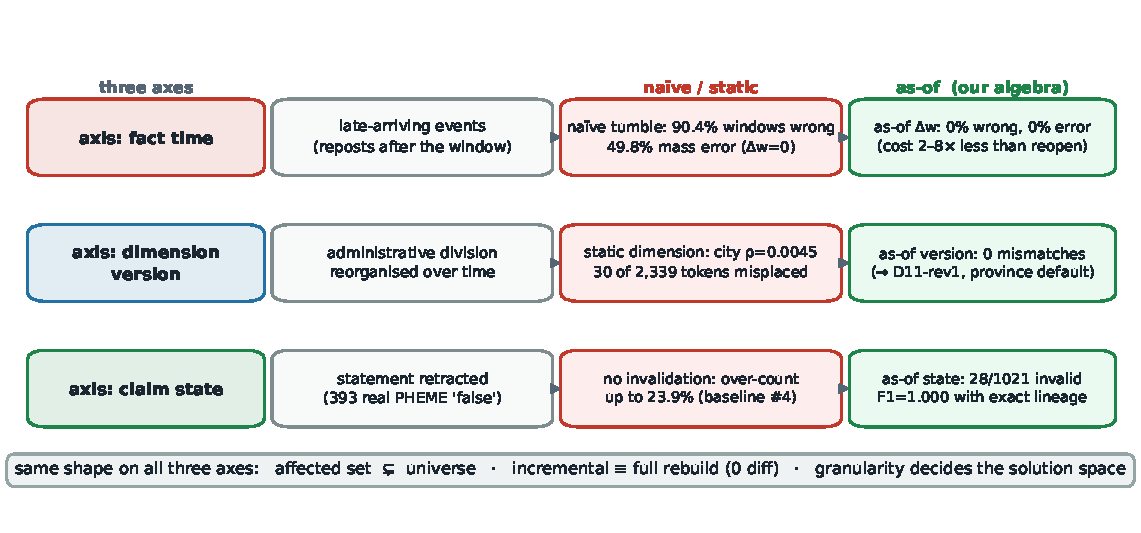
\includegraphics[width=0.88\columnwidth]{fig2_three_axis_asof.pdf}
\caption{Three axes, one shape. Each axis admits a na\"ive/static reading and
an as-of reading; the numbers are the measured outcomes of
\S7.2--\S7.4. All three share the same structure: the affected set is
a small fraction of the universe, incremental maintenance is bit-identical to
full rebuild, and representation granularity decides the solution space.}
\label{sfig:axes}
\end{figure}

\subsection*{Figure S2 · Real retraction over the PHEME false set (E5)}
\addcontentsline{toc}{subsection}{Figure S2 · Real retraction over the PHEME false set (E5)}
\noindent\emph{Referred to from the main paper, \S7.4.1.}

\begin{figure}[htbp]
\centering
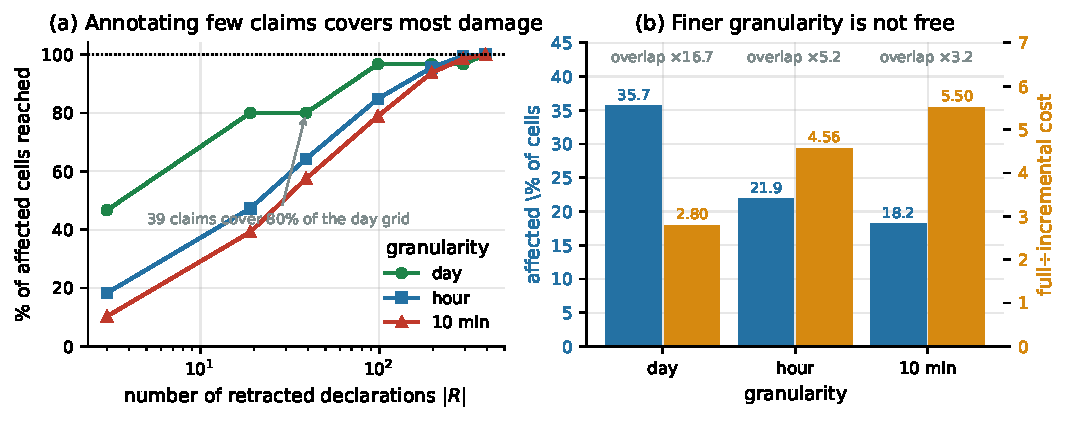
\includegraphics[width=0.88\columnwidth]{fig4_invalidation_coverage.pdf}
\caption{Real retraction over the PHEME \emph{false} set (E5). (a) Coverage of
the affected cell set as retractions accumulate: 39 of 393 claims already cover
80\% of the day-level affected set. (b) The granularity trade-off: finer
granularity shrinks the affected share but multiplies the
full$\div$incremental cost ratio.}
\label{sfig:invalid}
\end{figure}

\subsection*{Figure S3 · Calibrating the sparsity threshold (E12)}
\addcontentsline{toc}{subsection}{Figure S3 · Calibrating the sparsity threshold (E12)}
\noindent\emph{Referred to from the main paper, \S7.8.}

\begin{figure}[htbp]
\centering
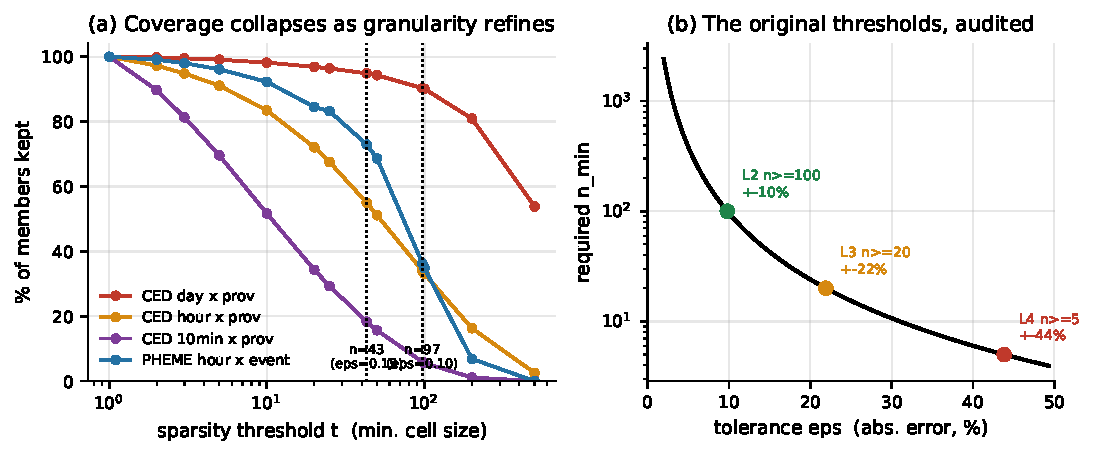
\includegraphics[width=0.88\columnwidth]{fig6_threshold_calibration.pdf}
\caption{Calibrating the sparsity threshold (E12). (a) Members kept by
qualified cells as the threshold grows: the same 1.09M posts lose coverage
rapidly as time granularity refines. (b) The required sample size
$n_{\min}(\varepsilon)\approx0.96/\varepsilon^2$ with the original D8
thresholds audited on the curve: L2 ${\ge}$100 sound, L3 ${\ge}$20 loose, L4
${\ge}$5 meaningless.}
\label{sfig:threshold}
\end{figure}



\section*{Appendix A: Design decisions behind the artefacts}
\addcontentsline{toc}{section}{Appendix A: Design decisions behind the artefacts}

The system is governed by 27 recorded decisions; the ones that shape the paper are: semantic dimensions generated in three hybrid layers (D1); retraction judged opportunistically from platform signals plus LLM adjudication, with full transition truth delegated to PHEME and Wikidata (D2, revised); frequency-layered measure representation (D3); coupled granularity across space/time/state (D4); community space demoted to a source attribute in stage one (D16); graph storage with tree roll-up and a seventh operation REPARENT (D7, D18); constellation schema $F_{\text{post}}+F_{\text{claim}}$ (D9); multi-role snowflaked geography with \textbf{province as the default granularity} (D10-rev1, D11-rev1, D14); versioned geography via CTAmap (D15); Wikidata as formal retraction truth (D21); availability as a veto criterion for data sources, and no dependence on a single platform API as a reproducibility claim (D23, D24).

\section*{Appendix B: Reproducibility checklist}
\addcontentsline{toc}{section}{Appendix B: Reproducibility checklist}

\begin{itemize}
\item \textbf{Data}: CED (codeload GitHub archive), CTAmap (Zenodo 10.5281/zenodo.22179207, CC-BY-4.0), PHEME (HF mirror + jsDelivr annotations), Wikidata (public SPARQL endpoint, query text and date stamped).
\item \textbf{Access channel}: \texttt{curl} subprocess + \texttt{--noproxy '*'}; retry policy documented; all queries carry a User-Agent with contact.
\item \textbf{Artefacts per experiment}: script, raw CSV, and a report with the exact discrepancy-checks (13 checkpoints, 3 granularities, 7 cross-checks, boundary verification in E9, and cell-for-cell 0-diff against the ablations in E10).
\item \textbf{Baseline-\#2 protocol (E14, EraRAG)}: the competitor is the public \texttt{EraRAG-Official} checkout, executed \textbf{CPU-only} (no GPU) with a local 384-d MiniLM embedding and a free-tier OpenAI-compatible LLM; every cost is reported as a \textbf{ratio} to a full rebuild measured on the same host in the same run, so no absolute token or wall-clock figure is claimed. Documents enter through the \emph{same} tweet$\to$chunk adapter used by every other experiment (snowflake id as the chunk title, raw text as the content), and the route actually taken (\texttt{\_build\_graph} vs \texttt{\_refine\_graph}) is recorded by a call-site probe rather than inferred from the resulting tree. The harness had to repair \textbf{13 defects} in the released code before it would run to completion; the list, the reasoning and a \texttt{git diff} patch are released. The stability result is re-tested in a \textbf{process-per-batch} mode in which each batch reloads the persisted tree before refining, so a crash cannot be attributed to in-memory state. The capability matrix is deterministic in its structural half (retriever enum, \texttt{mode\_list}, node-metadata keys, read from source) and behavioural in the rest (13 retrieval probes with context-survival rates, thread-purity and chance baselines, plus a refutation-injection contrast that re-indexes the 16 \texttt{disagreed} replies incrementally).
\item \textbf{Evaluation protocol (E11)}: all reported $Q_3$ numbers are \emph{out of sample}, stratified 5-fold cross-validation plus a temporal split by seed time; the "high-activity account" set that $S_{1a}$ depends on is recomputed from training folds only, so no test-fold statistic enters the features. E3's in-sample composite (0.664) is quoted only as the number our protocol replaces.
\item \textbf{Calibration protocol (E12)}: thresholds are derived, not tuned, $n_{\min}(\varepsilon)=\lceil z^2_{0.975}\cdot 0.25/\varepsilon^2\rceil$ (worst-case $p=0.5$), cross-checked against six real cube grids whose cell-size distributions and coverage curves are released verbatim; the cascade-size median (328) reproduces E10's independent measurement (327).
\item \textbf{Annotation protocol (E13, $Q_4$)}: the released protocol fixes the unit (a same-event assertion pair), a 4-class relation taxonomy one-to-one with \S5.4's measures, an \textbf{explicit decision order} over those classes and an explicit \textbf{slot key} $(\text{subject}\times\text{predicate}\times\text{time})$ with quantity excluded, a stratified sample with a per-event cap, a derivation of the sample size from E12's precision table, an inter-annotator gate ($\kappa\ge0.70$), met at \textbf{0.893} by full dual coverage rather than by 20\% overlap, since the probes are cheap, and a scorer reporting per-class P/R/F1 with a confusion matrix instead of accuracy. Annotators receive a \textbf{blinded} table only (\texttt{pair\_id / event / p\_text / q\_text}): the stratum name, the sampling prior and the PHEME veracity columns are withheld because they encode the answers. A 50-pair pilot was run with six independent fresh-context channels plus one arbitration; the codebook was frozen after four revisions ($\kappa$ 0.835 $\to$ 0.958, AC1 0.976) and both stratification priors were falsified (same-thread replies 92.3\% UNRELATED; opposite veracity $\to$ 0 conflicts), which is why the protocol's sampling is revised to add targeted DERIVE and CONFLICT layers. Tier-A anchors run without human input: the reply-tree ground truth, its 99.16\% \texttt{@}-mention witness rate, the content-channel recovery AUC (0.5005), and the 94 reciprocal Wikidata pairs. We also report that the claim-graph constructor's structural and content-only variants agree row for row (0/388), and that macro-F1 0.7315 is reported against a majority-class null of 0.1988 rather than accuracy. The protocol is then \textbf{executed}: a six-stratum, \textbf{582-pair} sample (the original four layers, pair-ids preserved, plus a cross-thread verbatim layer and a same-quantity-slot layer), a released \textbf{quantity-slot extractor} with its six guards, and an \textbf{out-of-sample yield probe} on 60 pairs under the frozen codebook. Yields are \textbf{94.4\%} for DERIVE and \textbf{11.1\%} for CONFLICT (strict 17.6\%, opposite-polarity 9.1\%, vague \textbf{0\%}) against a \textbf{2\%} random baseline; the codebook gains two explicit clauses (a leading mention is an \emph{addressee}, so a mention-only variant is DERIVE; a vague quantifier and a specific value are \emph{compatible}, so that sub-form is never a conflict), and the verbatim layer is split into \texttt{rt} / \texttt{mention-only} / \texttt{copy} (5 / 68 / 24) so that the 94.4\%-versus-16.7\% sensitivity of its yield is attributable rather than hidden. The quantity-slot rule is a \textbf{single-variable} change on top of the v1 constructor and leaves the 388-pair predictions identical per class. The codebook is then \textbf{closed} at five rulings ($A1$--$A5$): a leading mention is an addressee while \texttt{via @} / \texttt{source: @X} is an attribution (never DERIVE); quantity comparison first gates on \textbf{measure kind} (people / events / locations / vehicles / years, a mismatch is UNRELATED, not a conflict), then on total-versus-part (a part-marker must point at the \textbf{same measured population}; a lower bound on the larger side, or a definite sub-item \texttt{the \$N\$} on the smaller, also makes the readings compatible) versus total-versus-total (a conflict); and predicate mergeability is decided before quantity, with an explicit counter-example list for same-event-different-action families under the rule that \emph{sharing an event is not evidence of sharing an assertion}. The revision is validated on a 76-pair set (20 targeted-disagreement, 20 matched control, 36 fresh and disjoint) and the six prior disagreements plus six matched controls are re-checked after closure; the constructor is synced to the closed codebook as a third variant whose three guards are mechanisable (measure-kind gate, subset pass, attribution guard) and which is again single-variable with respect to the second; macro-F1 on the annotated set rises 0.5069 $\to$ 0.6333 (DERIVE F1 1.000, conflict precision 0.600, support still 0.118). The last unclosed ruling, predicate mergeability, is then \textbf{closed as a finite ten-family table} released as a CSV (family id, attribute, value, priority, surface forms, phrases): the table refines the measure classes into (attribute, value) pairs, life status (fatal / injured / victim-unspecified), custody (held / exited), perpetrator (exists / identity), force (gunfire / explosion), police action, and a pair is same-slot only if both quantities bind to the same family; otherwise it is UNRELATED, and if either side carries no family-valued quantity the ruling is \texttt{not-applicable} and falls through. Two binding laws and a \texttt{pred-out-of-table} ledger accompany it, and the ruling is re-implemented as a \textbf{fourth single-variable constructor variant} (macro-F1 0.6333 $\to$ 0.6764, conflict precision 0.600 $\to$ 1.000, original 388 pairs unchanged). Finally, the released verification attributes \textbf{each} of the 45 annotator-UNRELATED pairs to the clause that decides it (per-pair ids, single coder): non-propositionality 46.7\%, predicate non-mergeability 26.7\%, different event/entity 13.3\%, measure-kind 6.7\%, population 2.2\%, implicature 2.2\%. The protocol is then executed at \textbf{full scale}: a \textbf{755-pair, seven-stratum} sample (the 582-pair set retained pair-id-for-pair-id, the strict quantity layer extended from 97 to 233), labelled by \textbf{two independent full-coverage channels} split into four shards each, with a \textbf{third channel arbitrating the 46 disagreements} ($\kappa$ \textbf{0.8932}, AC1 0.8582) and a \textbf{fourth adjudicating the 5 items that split all three}; the released truth file keeps per-pair channel labels and a resolution column, so every label is traceable to its channel. Both yields replicate on disjoint data (DERIVE \textbf{94.8\%}, strict conflict \textbf{13.7\%} [9.9\%, 18.7\%], vague \textbf{0\%} a second time), giving \textbf{43} conflict labels and hence the first per-class conflict F1 (system macro-F1 \textbf{0.7109} vs a \textbf{0.1898} null; DERIVE 0.932, UNRELATED 0.892, SUPPORT 0.562, CONFLICT 0.457). The five all-channel splits are released as the control set for the next codebook revision, and the registered seams are priced rather than hidden (\textbf{0.40\%} for the lower-bound-direction family).
\item \textbf{Snapshot caveat}: WDQS reflects a live graph; the whole-graph count moved by +4 statements within 20 minutes during profiling. Any cited number must be accompanied by its query date.
\end{itemize}

\section*{Appendix C: The E13 annotation programme: full protocol and intermediate results}
\addcontentsline{toc}{section}{Appendix C: The E13 annotation programme: full protocol and intermediate results}

\emph{This appendix holds the procedural detail of the $Q_4$ semantic layer, moved out of \S7.4 so that the body reports outcomes rather than protocol history. Nothing here is new; every number also appears in \S7.4 in summarised form. It is included because the failures are as informative as the successes: the four codebook revisions, the two generators' out-of-sample yields, the full-set channel execution and the human test are what make the claim "the semantic layer is measurable but not yet settled" checkable rather than asserted.}

\textbf{The semantic layer is annotated, and the pilot falsifies our own stratification priors (E13 pilot).} We then ran the protocol on a 50-pair pilot, using an \emph{independent multi-channel probe} in place of human annotators: each channel reads only a \textbf{de-identified sample table} and the frozen codebook, in a fresh context, with no visibility of the others (six channels across two rounds plus one arbitration). Two hygiene points turned out to matter. First, the original sample table had to be \textbf{blinded}: its \texttt{stratum} column names (\texttt{S3\_...\_opposite\_veracity}) and its PHEME \texttt{veracity} columns are the \emph{answers} for the conflict layer, so shipping the raw table would have manufactured agreement; all channels see only \texttt{pair\_id / event / p\_text / q\_text}. Second, the codebook had to be revised four times, and the decisive fix was not more tag definitions but an explicit \textbf{decision order} (propositionality $\to$ implicature $\to$ slot/quantity $\to$ derivation $\to$ fallback) together with an explicit \textbf{slot key} $(\text{subject}\times\text{predicate}\times\text{time})$ with \emph{quantity explicitly excluded}. Under the v1.0 codebook the probe reaches $\kappa=0.835$ (4/50 disagreements); under the frozen v1.3 codebook it reaches $\kappa=\mathbf{0.958}$ ($p_o=0.980$, Gwet AC1 0.976, 1/50, arbitrated). Every revision was forced by a \emph{named} boundary family rather than by noise, and the last two rounds exposed a genuine oscillation on one question, \textbf{whether a numeric value is part of the slot key}, which decides whether "multiple suspects" versus "3 suspects" is SUPPORT or CONFLICT. We flag this because it is the same \emph{numeric-versus-semantic} fault line that runs through E10 and E12. We stress the epistemic status: the probe's channels share a backbone and the codebook was calibrated on the same 50 pairs, so this $\kappa$ is \textbf{optimistic and in-sample}; its legitimate use is \emph{falsification} (if independent channels cannot agree, the codebook is broken), not as a substitute for a human $\kappa$, and a human $\kappa$, measured later at full scale, is exactly what disqualifies this codebook (\S7.4).
\textbf{The pilot also falsifies two of our own stratification priors.} We had expected the same-thread reply layer to be rich in DERIVE/CONFLICT and the opposite-veracity layer to be a high-risk CONFLICT layer. Both expectations are wrong. Same-thread replies are \textbf{92.3\% (12/13) UNRELATED}: a structural reply edge carries no information about the semantic relation. And pairs whose threads carry \emph{opposite} veracity labels contain \textbf{zero} conflicts (0/12) versus 0/13 in the random control layer, a thread-level truth label is not an assertion-level conflict, so PHEME's veracity annotations cannot be repurposed as conflict supervision. The realized distribution is severely skewed: UNRELATED 66\%, SUPPORT 28\%, DERIVE 4\%, CONFLICT 2\%. This has a direct evaluation consequence that we state rather than hide: at $n{=}50$ the two minority classes cannot support per-class statistics, and extrapolating the pilot to the full 388-pair sample would yield roughly 15 DERIVE and 8 CONFLICT pairs, not enough to interpret a per-class F1. The protocol therefore revises its sampling (v1.1): the original four layers are retained but re-assigned as negative controls and a baseline, and two \textbf{targeted} layers are added, an RT/quote layer for DERIVE and a same-slot mutually-exclusive-value layer for CONFLICT. The second one has a cost we now accept explicitly: \textbf{without slot (subject--predicate) matching one cannot sample conflicts at all}, so extraction, previously out of scope, becomes a prerequisite for evaluating the CONFLICT class.
\textbf{We then built both targeted layers and measured their yield out of sample, with the codebook frozen in advance.} This distinction matters: the pilot's $\kappa$ was calibrated in-sample, whereas the yield probe below was run on 60 pairs that never participated in any codebook revision, so it is an out-of-sample quantity. The DERIVE layer is a cross-thread near-verbatim generator (character 3-gram coverage $\ge0.90$ after removing mentions and URLs); the CONFLICT layer is a \textbf{quantity-slot} generator, where a \emph{slot} is the projection of the codebook's slot key onto the one layer T5 actually operates on, $(\text{measure head-class},\ \text{value set})$, with head classes restricted to entity counts (dead, injured, hostage, suspect, airplane, building) and six guards derived from observed false positives (numbers in time/age/unit contexts, four-digit years, interposed prepositions, typographic numerics such as \texttt{b4} or \texttt{1st}, implausible magnitudes, and a whitelist for the reverse "death toll rose to $N$" pattern). The yield gap is stark: \textbf{94.4\%} of the DERIVE-layer pairs are labelled DERIVE (17/18, 95\% Wilson [74.2\%, 99.0\%]), versus \textbf{11.1\%} for the CONFLICT layer (4/36), 17.6\% in its strict sub-form (both sides purely numeric and disjoint), 9.1\% for same-slot opposite-polarity, and \textbf{0\%} for the vague-quantifier sub-form, whose five-of-eight items the annotators instead call SUPPORT or UNRELATED. That last number is not a failure but a confirmation: T5 (quantity compatibility) says a vague quantifier and a specific value \emph{can} hold simultaneously, and the annotators agree, which is also how we caught, and removed, the single regression that quantity-slot reasoning introduced into the constructor (the \texttt{multiple suspects} versus \texttt{3 suspects} pair, the very case on which the codebook had oscillated). Relative to a 2\% random-stratum baseline, the strict generator is \textasciitilde{}9$\times$ denser; at that yield, reaching 30 labelled CONFLICT pairs requires a \textbf{$\approx$170-pair} strict layer, a size we derive from E12's precision table rather than assert. \textbf{Surface quantity conflict is abundant, 96,954 candidate pairs, but its semantic yield is \textasciitilde{}9$\times$ lower}, which is why we report candidate-pool size and yield separately throughout. We then closed the four codebook boundaries the probe exposed and \textbf{re-measured on a fresh, disjoint 36-pair S6 batch} so the quantity stays out-of-sample: yield falls to \textbf{5.9\%} overall (2/34, 95\% Wilson [1.6\%, 19.1\%]) and \textbf{11.1\%} strict ([3.1\%, 32.8\%]), with opposite-polarity now \textbf{0\%} and the vague sub-form still 0\%. The direction is by construction, the new A3 clause removes \emph{subset} pairs from conflict, and a subset pair was previously scored as a quantity conflict, while the magnitude is not significant at this $n$ (the two Wilson intervals overlap), so we report both. The cost consequence is concrete: 30 labelled conflicts now need \textbf{$\approx$270} strict pairs. Because none of the twelve re-checked pairs is a conflict under either reading, this refinement does not disturb the out-of-sample yield measurement. \textbf{We then paid the cost} the figure implies: the full annotation set was scaled to \textbf{755 pairs} (the strict layer extended from 97 to 233) and annotated end to end, which delivers \textbf{43} conflict labels and with them the first per-class conflict F1 (next two paragraphs).
\textbf{A measured yield is only as stable as the codebook clause that defines it, and one clause dominates.} Of the DERIVE layer's 97 candidates, \textbf{68 (70.1\%)} differ \emph{only} in their leading \texttt{@mention}: after removing mentions and URLs the two texts are byte-identical. The frozen codebook computes coverage after removing mentions, so the correct label is DERIVE and the yield is 94.4\%; had one classed the leading mention as a \emph{source change} instead, the same rule would have produced 16.7\%. Both independent channels flagged this seam unprompted. We therefore write the clause down explicitly: a leading mention is an \emph{addressee}, not part of the proposition, and split the layer into \texttt{rt} / \texttt{mention-only} / \texttt{copy} sub-forms (5 / 68 / 24) so that the sensitivity can be reported per sub-form rather than hidden inside an aggregate. The episode generalises: when an annotation-derived metric swings by a factor of five on one classification clause, the clause, not the sample size, is the binding constraint.
\textbf{Revising a codebook must be tested against both its targets \emph{and} its controls, and our first attempt failed the control.} Fixing the two remaining seams as explicit rulings (A3/A4: quantity measure-kind before total-versus-part; predicate mergeability with a worked counter-example list) converged \textbf{5 of 6} prior disagreements on a 76-pair verification set (20 targeted, 20 matched controls drawn from previously-agreed pairs, 36 fresh) at $\kappa=0.871$ (95\% CI 0.764--0.958, AC1 0.901). But it also \textbf{broke two control pairs that had been agreed}, and, on inspection, \emph{both} breakages were caused by the new wording itself: \texttt{of six hostages} was accepted as a "part" of a post about \emph{shooting deaths} (the part-marker was not required to point at the same population the first post quantified), and \texttt{via @theblaze} was stripped as if it were an addressee because the addressee clause had been written as "remove mentions, then compare", which silently swallowed \emph{attribution}. Had we measured convergence alone, we would have declared the revision a success. The correction is four wording changes and no new concepts, measure-kind is promoted to a \emph{gate} before the total-versus-part test, the part-marker must point at the same population, the same-event-different-action family is written out as a counter-example list with the rule "sharing an event is not evidence of sharing an assertion", and the two roles of \texttt{@} are separated (leading mention = addressee $\Rightarrow$ DERIVE after stripping; \texttt{via @} / \texttt{source: @X} = attribution $\Rightarrow$ never DERIVE). On a re-check set of exactly the six prior disagreements plus six matched controls, all six converge and all six controls hold with zero label drift. We state the epistemic status plainly: that re-check is \textbf{in-sample}, the six items are precisely the ones the revision targeted, so a perfect score there is not evidence that the codebook is good; the control block can only show that nothing was broken. The single independent check remains a human $\kappa$ on a held-out sample.
\textbf{Structure supplies the edge; it does not supply the type.} Our claim-graph constructor (\S5.4) is a rule-based predictor with an eight-rule ladder (RT/containment, character 3-gram overlap, polarity, numeric exclusivity, containment thresholds), implemented in two variants: with the platform reply edge available, and content-only. Across all 388 pairs the two variants agree \textbf{row for row} (0 differences; the structural relaxations only widen two thresholds, and both bands are empty). Combined with A2 (content cannot recover the edge), this is a complete irreducibility statement for $Q_4$: \textbf{the edge must come from the platform, the type must come from annotation, and neither can be inferred from the other.} It also sharpens the cost of D24: discarding platform structure loses the edge irrecoverably, but \emph{keeping} it still buys nothing for the type. On the pilot, the constructor reaches macro-F1 \textbf{0.7315} against a majority-class null of \textbf{0.1988}; however only SUPPORT (P 1.00 / R 0.571) and UNRELATED (P 0.861 / R 0.939) are interpretable at this sample size, the DERIVE and CONFLICT columns being single-digit support. As in E6, we report the macro figure and not accuracy, because the null baseline's accuracy is already 0.66. The quantity-slot rule is introduced as a \textbf{single-variable change} (polarity and RT definitions are held from v1), which makes the comparison clean: on the original 388 pairs the two versions are \textbf{identical per class}, the rule neither helps nor harms where it was never designed to apply, while adding CONFLICT capability on the targeted layer. On the targeted subset itself, however, the constructor's macro-F1 falls to \textbf{0.5304}, with \textbf{zero} SUPPORT predictions: its SUPPORT rule is purely lexical, and the targeted pairs are low-overlap by construction. The interface works; the capability is bounded. Report the two numbers together and the constructor looks weak; report only the first and the bound disappears. \textbf{Syncing the constructor to the closed codebook makes the bound explicit rather than implicit.} Three mechanisable guards implement A3 and A5, a measure-kind gate (a count followed by \texttt{situations/attacks/incidents/locations} is a count of \emph{events}, not of people, so the quantity slots are not comparable), a subset pass (a numeric clash is not a conflict when a part-marker points at the same measured population, when the larger side is a lower bound, or when the smaller side is a definite sub-item \texttt{the \$N\$}), and an attribution guard (a source marker present in the later post but not the earlier one forbids DERIVE, and \texttt{via @} no longer counts as a verbatim-echo trace). Thresholds and every definition outside those guards are held fixed, so the change is single-variable again. On the 76-pair annotated set macro-F1 rises from \textbf{0.5069} to \textbf{0.6333}: DERIVE reaches \textbf{P = R = F1 = 1.000}, conflict precision goes \textbf{0.250 $\to$ 0.600}, UNRELATED 0.758 $\to$ 0.816, and \textbf{SUPPORT stays at F1 0.118}, because a purely lexical support rule cannot see a same-claim paraphrase that shares no content words. On the original 388 pairs the guards move 9 predictions (conflict 11 $\to$ 9, DERIVE 25 $\to$ 20, support 62 $\to$ 68), which is the expected consequence of a stricter codebook rather than a regression.
\textbf{Closing the last free choice converts a counter-example list into a table, and makes the criterion's binding clause measurable.} Four of the five rulings are mechanically checkable; predicate mergeability was not, because it was stated as an enumerative list of same-event-different-action families. We close it by refining the \emph{measure} abstraction: the slot extractor's head classes (\texttt{hostage}, \texttt{suspect}, \ldots{}) are too coarse for the ruling, since they merge "held hostage" with "hostages escaped", and "an armed suspect exists" with "the suspect's biography". A predicate family is therefore an (attribute, value) pair, ten in total, spanning life status (fatal / injured / victim-unspecified), custody status (held / exited), perpetrator (exists / identity), force (gunfire / explosion) and police action, and two quantities are comparable only if they bind to the \emph{same} family; otherwise the pair is UNRELATED. Two ordering laws make the binding determinate: measure over generalisation (as before), and a \textbf{state-transition predicate over the static noun argument it governs}, \texttt{5 hostages escaped} binds to \texttt{CUSTODY\_EXITED}, not \texttt{CUSTODY\_HELD}, and inverting this is exactly what our own self-test caught first. A third, \texttt{not-applicable} state is required rather than optional: if either side carries no family-valued quantity the ruling does not apply and the decision falls through, because treating "no quantity" as UNRELATED would have destroyed 95 of the 97 verbatim-layer pairs. On the 76-pair annotated set the ruling applies to \textbf{82.9\%} of pairs; it passes \textbf{19/19 (100\%)} of the pairs the annotators call same-slot, blocks 27.3\% of the applicable UNRELATED pairs, and reproduces \textbf{9/9} of the boundary families named by the codebook, up from 5/9. Synced as a single mechanisable guard on top of the third constructor, macro-F1 rises \textbf{0.6333 $\to$ 0.6764}, conflict precision \textbf{0.600 $\to$ 1.000} (F1 0.600 $\to$ 0.750) and UNRELATED recall 0.933 $\to$ 0.978, while the original 388 pairs are unchanged line for line.
\textbf{Now that the ruling is finite, we can ask which clause actually decides each UNRELATED pair}, a question the codebook could not previously answer, and one that re-allocates annotation effort. All 45 UNRELATED pairs in the annotated set are attributable (single-coder; per-pair ids released with the artefacts): \textbf{T1 non-propositionality (questions, imperatives, opinion, speculation) accounts for 46.7\%}, predicate non-mergeability for \textbf{26.7\%}, different-event/entity for 13.3\%, measure-kind mismatch for 6.7\%, population mismatch for 2.2\% and implicature for 2.2\%. The practical reading is that closing predicate mergeability was worth doing: it removes the last unclosed clause and is what takes conflict precision to 1.000, but \textbf{the dominant constraint is whether a post asserts anything at all}. This is the same style of attribution that told us, in the yield probe, that one clause could swing a metric by 5.7$\times$; here it tells us where the annotation disagreements will actually be.
\textbf{Scaling the probe to the full set converts the semantic layer from a protocol into a measurement, and it replicates the yields that motivated the sampling in the first place.} The full sample is \textbf{755 pairs} (S1--S4 at 97 each retained unchanged, the verbatim layer at 97, the slot layer extended to 270 with 233 strict), labelled by \textbf{two independent full-coverage channels} split into four shards each, with a \textbf{third channel} arbitrating the disagreements and a \textbf{fourth} adjudicating the five items on which all three disagreed. Agreement is \textbf{93.9\% with $\kappa=0.8932$} (AC1 0.8582; 46 disagreements, 6.1\%), and the per-layer structure is informative: the verbatim layer is \textbf{100\% agreed (97/97, $\kappa=1.000$)}, no channel, unprompted, re-opened the addressee clause that the 5.7$\times$ sensitivity had forced us to write down, whereas the same-thread reply layer, the weakest prior in the pilot, remains the least reliable at $\kappa=0.553$. The realized distribution is \textbf{UNRELATED 462 / SUPPORT 145 / DERIVE 105 / CONFLICT 43}, and the two targeted layers replicate the pilot on disjoint data: \textbf{94.8\%} DERIVE (92/97, pilot 94.4\%), \textbf{13.7\%} conflict in the strict layer (32/233, 95\% Wilson [9.9\%, 18.7\%], pilot 11.1\%, intervals overlapping) and \textbf{0\%} for the vague sub-form a second time. The two layers also remain mutually exclusive in what they produce: the verbatim layer yields \textbf{no} conflict and the slot layer yields \textbf{no} DERIVE, which is the sampling analogue of the two-layer measure argument in \S7.7. With \textbf{43} conflicts the class clears the $n\ge 30$ interpretability gate derived from E12, so all four classes are reportable. Evaluated on this full truth set, the fourth constructor reaches \textbf{macro-F1 0.7109} against a majority-class null of \textbf{0.1898}, with per-class F1 of \textbf{0.932} (DERIVE, $n{=}105$), \textbf{0.892} (UNRELATED, $n{=}462$), \textbf{0.562} (SUPPORT, $n{=}145$) and \textbf{0.457} (CONFLICT, $n{=}43$, P 0.593 / R 0.372). Two things must be read together with that table. First, the two easy classes carry the macro figure; the two hard ones expose the rule-based boundedness already visible on the targeted subset, a lexical support rule cannot see a paraphrase, and a value-exclusivity conflict rule catches only one morphology of disagreement. Second, conflict \textbf{precision falls from 1.000 at $n{=}6$ to 0.593 at $n{=}43$}: the pilot's perfect precision was a small-sample artefact, which is precisely the lesson E12 encodes and which we now demonstrate on the system side rather than only the annotation side.
\textbf{The residual disagreement is not noise; it localises the one seam the codebook never closed.} Of 755 pairs only \textbf{five} split all three channels, and \textbf{three of those five are a single family}: a lower-bound or hedged marker against a specific smaller value (\texttt{at least five hostages} vs \texttt{1 hostage}; \texttt{1 shooter} vs \texttt{possible five shooters}). The codebook's A3 clause forbids conflicts when the larger value carries a subset/lower-bound marker, but it never states the \emph{direction} in which such a marker licenses compatibility, and A2's "vague and specific are compatible" is likewise silent on it, which is exactly the subset-versus-total seam registered when the probe was left open, and which the fourth channel resolved to conflict with a written reason. The remaining two items belong to the second registered seam (sharing an event is not sharing an assertion: a shooting count of 2 vs 3; "no survivors expected" vs a passenger manifest). We deliberately do \textbf{not} amend v1.6 \emph{in place} for these: it is the version the 755 labels were produced under, and silently rewriting it would void them, any revision must instead be re-judged independently on every pair it can touch, which is the procedure the next three paragraphs use. Instead the seam is bounded and priced, \textbf{3 of 755 = 0.40\%}, and the five items are carried forward as ready-made controls for the next revision. The generalisable point is that a frozen codebook, once executed at scale, tells you where its own residual freedom lives, and that location is measurable rather than guessed.
\textbf{The probe can be falsified by a human, and the first human test disqualifies the v1.6 codebook.} The protocol's own hygiene rule (Threats 8--9) is that inter-channel agreement shows only that a codebook is \emph{executable}, never that it matches human judgement; the open quantity was a human $\kappa$. We measured it with a \textbf{single-annotator, two-pass} blind annotation of \textbf{48 items} drawn by stratified sampling over the four labels (DERIVE 10 / SUPPORT 12 / CONFLICT 12 / UNRELATED 14; CONFLICT over-sampled because it is 5.7\% of the pool), answered first \textbf{by intuition} with no guide and then \textbf{under the frozen codebook}. The decision rule was pre-registered: guided $\kappa\ge0.80$ with intuitive $\kappa\ge0.60$ is adequate; guided $\kappa\ge0.80$ but intuitive $<0.60$ means the codebook is counter-intuitive; \textbf{guided $\kappa<0.80$ means the codebook has holes and must be revised}. The outcome is the third: intuitive $\kappa=\mathbf{0.3945}$ (95\% CI 0.216--0.575) rising only to guided $\kappa=\mathbf{0.4959}$ (CI 0.315--0.661). The guide \emph{helps}, macro-F1 0.542 $\to$ \textbf{0.602}, UNRELATED recall 0.429 $\to$ \textbf{0.786}, and the dominant "same event $\Rightarrow$ SUPPORT" error is more than halved, but it does not make the task human-reproducible. Crucially the disagreement \textbf{localises} rather than diffuses: three families account for 64\% of the 22 intuitive-pass disagreements, each traceable to a single named clause, reading \emph{sharing an event} as support (6), reading high lexical overlap as derivation without checking for a citation trace (5), and insensitivity to incompatibility (5). Two qualifications bound the reading: the annotator is the \textbf{designer}, so this is a \emph{knowledgeable} human and the $\kappa$ is a \textbf{lower bound}, and the 48-item interval is wide. The instructive part is the cross-check, replaying the frozen v4 codebook on the 18 items the human judged wrongly, \textbf{the system is wrong on 12 of them}. The holes therefore exist at \textbf{both} layers, the \emph{codebook text} and the \emph{mechanical rule}, not in a human who merely failed to read the guide. This is the falsification the pilot could not perform, and it forces a revision.



% 由 gen_refs_tex.py 生成 —— 勿手改。
% 编号与 主论文_submission_v1.md 的 References 完全一致。
\begin{thebibliography}{99}

\bibitem{r1} Edge, Darren, Trinh, Ha, Cheng, Newman, Bradley, Joshua, Chao, Alex, Mody, Apurva, Truitt, Steven, and Larson, Jonathan. From Local to Global: A Graph RAG Approach to Query-Focused Summarization. 2024.

\bibitem{r2} Z. Guo, L. Xia, et al. LightRAG: Simple and Fast Retrieval-Augmented Generation. In \emph{EMNLP Findings 2025}, 2025. DOI: \url{https://doi.org/10.18653/v1/2025.findings-emnlp.568}

\bibitem{r3} F. Zhang, Z. Huang, Y. Zhou, X. Zhou, et al. EraRAG: Efficient and Incremental Retrieval Augmented Generation for Growing Corpora. arXiv:2506.20963, 2025. DOI: \url{https://doi.org/10.48550/arXiv.2506.20963}

\bibitem{r4} Zubiaga, Arkaitz, Aker, Ahmet, Bontcheva, Kalina, Liakata, Maria, and Procter, Rob. Detection and Resolution of Rumours in Social Media: A Survey. \emph{ACM Computing Surveys}, 51(2):32:1–32:36, 2018. DOI: \url{https://doi.org/10.1145/3161603}

\bibitem{r5} Zubiaga, Arkaitz, Liakata, Maria, Procter, Rob, Wong Sak Hoi, Geraldine, and Tolmie, Peter. Analysing How People Orient to and Spread Rumours in Social Media by Looking at Conversational Threads. \emph{PLoS ONE}, 11(3):e0150989, 2016. DOI: \url{https://doi.org/10.1371/journal.pone.0150989}

\bibitem{r6} Liu, Zhiyuan, Zhang, Le, Tu, Cunchao, and Sun, Maosong. Statistical and Semantic Analysis of Rumors in Chinese Social Media. \emph{Scientia Sinica Informationis}, 45(12):1536–1546, 2015.

\bibitem{r7} Kimball Group. Slowly Changing Dimensions. The Data Warehouse Toolkit: Dimensional Modeling Techniques, 2008.

\bibitem{r8} C. X. Lin, B. Ding, J. Han, F. Zhu, and B. Zhao. Text Cube: Computing IR Measures for Multidimensional Text Database Analysis. In \emph{ICDM 2008}, 2008. DOI: \url{https://doi.org/10.1109/ICDM.2008.135}

\bibitem{r9} D. Zhang and C. Zhai. MiTexCube: MicroTextCluster Cube for online analysis of text cells and its applications. \emph{Statistical Analysis and Data Mining}, 2012. DOI: \url{https://doi.org/10.1002/sam.11159}

\bibitem{r10} J. Han, Y. Chen, G. Dong, et al. Stream Cube: An Architecture for Multi-Dimensional Analysis of Data Streams. \emph{Distributed and Parallel Databases}, 2005. DOI: \url{https://doi.org/10.1007/s10619-005-3296-1}

\bibitem{r11} C. Bernard. Immersing evolving geographic divisions in the Semantic Web (Theseus Framework). 2019.

\bibitem{r12} Paolo Buonanno, Bianca Cattaneo, Giampaolo Lecce, Vitantonio Mariella, and Laura Ogliari. Building Consistent Territorial Units over Time: A Graph-Based Method for Historical Municipal Boundaries in Italy. 2025.

\bibitem{r13} 王春玲, 诸云强, 王曙, 刘纪猛, 冯敏, and 高振记. 考虑时空特征及演化关系的行政区划知识图谱构建. \emph{地球信息科学学报}, 28(1):89–104, 2026.

\bibitem{r14} Y. Cheng, Y. Hu, et al. A continuous vector dataset of Chinese administrative divisions from 2000 to 2026. 2025. DOI: \url{https://doi.org/10.5281/zenodo.22179207}

\bibitem{r15} Vrandečić, Denny and Kr{\"o}tzsch, Markus. Wikidata: A Free Collaborative Knowledgebase. \emph{Communications of the ACM}, 57(10):78–85, 2014. DOI: \url{https://doi.org/10.1145/2629489}

\bibitem{r16} F. Tao, C. Zhang, X. Chen, and J. Han. Doc2Cube: Allocating Documents to Text Cube Without Labeled Data. In \emph{ICDM 2018}, 2018. DOI: \url{https://doi.org/10.1109/ICDM.2018.00169}

\bibitem{r17} S. R. Surve. VectorCube: Multi-Granular Neuro-Symbolic Data Cubes for Semantic OLAP. In \emph{CSIT 2026}, 2026. DOI: \url{https://doi.org/10.5121/csit.2026.160203}

\bibitem{r18} X. Liu and L. Yang. LLM-Assisted Conversational Navigation over Multidimensional Data Cubes (NavLLM). \emph{Expert Systems with Applications}, 2026. DOI: \url{https://doi.org/10.1016/j.eswa.2026.132958}

\bibitem{r19} D. Maio and S. Rizzi. Bridging OLAP and RAG: A Multidimensional Approach to the Design of Corpus Partitioning. arXiv:2601.03748, 2026. DOI: \url{https://doi.org/10.48550/arXiv.2601.03748}

\bibitem{r20} D. Zhang and C. Zhai. Topic Cube: Topic Modeling for OLAP on Multidimensional Text Databases. In \emph{SDM 2009}, 2009. DOI: \url{https://doi.org/10.1137/1.9781611972795.96}

\bibitem{r21} L. Oukid and O. Boussaid. TLabel: A New OLAP Aggregation Operator in Text Cubes. In \emph{RCIS 2016}, 2016.

\bibitem{r22} L. Oukid, O. Asfari, et al. CXT-cube: contextual text cube model and aggregation operator for text OLAP. In \emph{RCIS 2013}, 2013.

\bibitem{r23} 侯东风, 张维明, 刘青宝, and 邓苏. 基于兴趣视图子集的流立方体计算方法. \emph{计算机研究与发展}, 2011.

\bibitem{r24} 袁正午, 程宇翔, 梁均军, and 李林. 一种高效流立方体结构. \emph{计算机工程与应用}, 2011.

\bibitem{r25} 尹为, 张成虎, and 甘凯. 基于数据流多维分析的可疑金融交易动态识别. \emph{北京理工大学学报（社会科学版）}, 2013.

\bibitem{r26} A. Cuzzocrea, C. De Maio, et al. OLAP analysis of multidimensional tweet streams for supporting advanced analytics. In \emph{ACM SAC 2016}, 2016. DOI: \url{https://doi.org/10.1145/2851613.2851662}

\bibitem{r27} N. U. Rehman, A. Weiler, and M. Scholl. OLAPing social media. In \emph{ASONAM 2013}, 2013. DOI: \url{https://doi.org/10.1145/2492517.2500273}

\bibitem{r28} M. Ben Kraiem, M. A. Alqarni, et al. OLAP operators for social network analysis. \emph{Cluster Computing}, 2019. DOI: \url{https://doi.org/10.1007/s10586-019-03006-z}

\bibitem{r29} Y. Huang, S. Zhang, et al. KET-RAG: A Cost-Efficient Multi-Granular Indexing Framework for Graph-RAG. In \emph{KDD 2025}, 2025. DOI: \url{https://doi.org/10.1145/3711896.3737012}

\bibitem{r30} T. Bian, X. Xiao, et al. Rumor Detection on Social Media with Bi-Directional Graph Convolutional Networks. In \emph{AAAI 2020}, 2020. DOI: \url{https://doi.org/10.1609/aaai.v34i01.5393}

\bibitem{r31} T. Chen, X. Li, et al. Call Attention to Rumors: Deep Attention Based Recurrent Neural Networks for Early Rumor Detection. In \emph{PAKDD 2018}, 2018. DOI: \url{https://doi.org/10.1007/978-3-030-04503-6_4}

\bibitem{r32} R. Xia, K. Xuan, and J. Yu. A State-independent and Time-evolving Network for Early Rumor Detection in Social Media. In \emph{EMNLP 2020}, 2020. DOI: \url{https://doi.org/10.18653/v1/2020.emnlp-main.727}

\bibitem{r33} Y. C. Wu, J. Sun, et al. Dual-channel early rumor detection based on factual evidence. \emph{Expert Systems with Applications}, 2023. DOI: \url{https://doi.org/10.1016/j.eswa.2023.121928}

\bibitem{r34} F. Zeng, Q. Shao, et al. LLM-based early rumor detection with imitation agent. SMU InK, 2026.

\bibitem{r35} Stuart E. Middleton and Vadims Krivcovs. Geoparsing and Geosemantics for Social Media: Spatiotemporal Grounding of Content Propagating Rumors to Support Trust and Veracity Analysis during Breaking News. \emph{ACM TOIS 34(3)}, 1–26, 2016. DOI: \url{https://doi.org/10.1145/2842604}

\bibitem{r36} S. M. Fitzhugh, C. Butts, et al. Spatio-temporal filtering techniques for the detection of disaster-related communication. \emph{Social Science Research}, 2016. DOI: \url{https://doi.org/10.1016/j.ssresearch.2016.04.023}

\bibitem{r37} Sean M. Fitzhugh. The Spacetime Continuum: Using Spatio-temporal Filtering Techniques to Revisit Rumor Theory. 2015.

\bibitem{r38} Hongyu Wang, Ke Li, and Shuo Shang. DLRD: dual-level network for rumor detection on geo-textual data. \emph{GeoInformatica 28(2)}, 335–351, 2024. DOI: \url{https://doi.org/10.1007/s10707-023-00505-5}

\bibitem{r39} Chunyang Jiang, Bing Wang, Jianfeng Qu, and Ximing Li. Geo-textual rumor detection in location-based social media by decomposing spatial subspaces. \emph{GeoInformatica 30}, Article 20, 2026. DOI: \url{https://doi.org/10.1007/s10707-026-00579-x}

\bibitem{r40} M. Kaufmann, P. M. Fischer, et al. TPC-BiH: A Benchmark for Bitemporal Databases. In \emph{TPCTC 2013}, 2014. DOI: \url{https://doi.org/10.1007/978-3-319-04936-6_2}

\bibitem{r41} Doyle, Jon. A Truth Maintenance System. \emph{Artificial Intelligence}, 12(3):231–272, 1979. DOI: \url{https://doi.org/10.1016/0004-3702(79})90008-0

\bibitem{r42} R. Bliujute, S. Šaltenis, et al. Systematic Change Management in Dimensional Data Warehousing. 1998.

\bibitem{r43} T. M. Nguyen and A Min Tjoa. An approach towards an event-fed solution for slowly changing dimensions in data warehouses with a detailed case study. \emph{Data \& Knowledge Engineering}, 2006. DOI: \url{https://doi.org/10.1016/j.datak.2006.10.004}

\bibitem{r44} Z. Li, X. Jin, et al. Temporal Knowledge Graph Reasoning Based on Evolutional Representation Learning (RE-GCN). In \emph{SIGIR 2021}, 2021. DOI: \url{https://doi.org/10.1145/3404835.3462963}

\bibitem{r45} Z. Li, S. Guan, et al. Complex Evolutional Pattern Learning for Temporal Knowledge Graph Reasoning. In \emph{ACL 2022}, 2022. DOI: \url{https://doi.org/10.18653/v1/2022.acl-short.32}

\bibitem{r46} B. Chen, C. Xiao, et al. Natural Evolution-based Dual-Level Aggregation for Temporal Knowledge Graph Reasoning. In \emph{EMNLP Findings 2024}, 2024. DOI: \url{https://doi.org/10.18653/v1/2024.findings-emnlp.543}

\bibitem{r47} R. Xu, Z. Qi, et al. Knowledge Conflicts for LLMs: A Survey. In \emph{EMNLP 2024}, 2024. DOI: \url{https://doi.org/10.18653/v1/2024.emnlp-main.486}

\bibitem{r48} S. Wang, Y. Zhu, et al. Knowledge Editing for Large Language Models: A Survey. \emph{ACM Computing Surveys}, 2024. DOI: \url{https://doi.org/10.1145/3698590}

\bibitem{r49} B. Zhang, Z. Chen, et al. LOKA: Conflict-Aware LLM Knowledge Update with Adaptive Knowledge Memory. In \emph{ACL 2026}, 2026. DOI: \url{https://doi.org/10.18653/v1/2026.acl-long.760}

\bibitem{r50} Cormode, Graham and Muthukrishnan, S. An Improved Data Stream Summary: The Count-Min Sketch and Its Applications. \emph{Journal of Algorithms}, 55(1):58–75, 2005. DOI: \url{https://doi.org/10.1016/j.jalgor.2003.12.001}

\bibitem{r51} Karnin, Zohar, Lang, Kevin, and Liberty, Edo. Optimal Quantile Approximation in Streams. In \emph{Proc. 57th IEEE Annual Symposium on Foundations of Computer Science (FOCS)}, pp. 71–78, 2016. DOI: \url{https://doi.org/10.1109/FOCS.2016.17}

\bibitem{r52} Flajolet, Philippe, Fusy, Éric, Gandouet, Olivier, and Meunier, Frédéric. HyperLogLog: The Analysis of a Near-Optimal Cardinality Estimation Algorithm. In \emph{Proc. Int. Conf. on Analysis of Algorithms (AofA), DMTCS Proceedings}, pp. 127–146, 2007. DOI: \url{https://doi.org/10.46298/dmtcs.3545}

\bibitem{r53} Kane, Daniel M., Nelson, Jelani, and Woodruff, David P. On the Exact Space Complexity of Sketching and Streaming Small Norms. In \emph{Proc. 21st Annual ACM-SIAM Symposium on Discrete Algorithms (SODA)}, pp. 1161–1178, 2010.

\bibitem{r54} H. Xu, Magdalen Dobson Manohar, et al. In-Place Updates of a Graph Index for Streaming Approximate Nearest Neighbor Search. arXiv:2502.13826, 2025. DOI: \url{https://doi.org/10.48550/arXiv.2502.13826}

\bibitem{r55} F. Zhang, M. Jiang, et al. Efficient Dynamic Indexing for Range Filtered Approximate Nearest Neighbor Search. In \emph{SIGMOD/PACMMOD 2025}, 2025. DOI: \url{https://doi.org/10.1145/3725401}

\bibitem{r56} Z. Wu, J. Jin, et al. MERIT: Efficient In-Place Deletion for Dynamic Graph-Based Approximate Nearest Neighbor Indexes. arXiv:2607.29173, 2026. DOI: \url{https://doi.org/10.48550/arXiv.2607.29173}

\bibitem{r57} D. Lee and M.-S. Kim. CONDA: A Connectivity-Aware Dynamic Index for Approximate Nearest Neighbor Search over Evolving Data. In \emph{VLDB 2026}, 2026. DOI: \url{https://doi.org/10.14778/3836663.3836694}

\bibitem{r58} Z. Zhang, Y. Wei, et al. CleanANN: Efficient and Robust Full Dynamism in Graph-based Approximate Nearest Neighbor Search. In \emph{SPAA 2026}, 2026. DOI: \url{https://doi.org/10.1145/3816782.3819219}

\bibitem{r59} 李琪 and 白英彩. 数据仓库中时态视图的维护. \emph{软件学报}, 2002.

\bibitem{r60} Harinarayan, Venky, Rajaraman, Anand, and Ullman, Jeffrey D. Implementing Data Cubes Efficiently. In \emph{Proc. 1996 ACM SIGMOD Int. Conf. on Management of Data}, pp. 205–216, 1996. DOI: \url{https://doi.org/10.1145/233269.233333}

\bibitem{r61} Green, Todd J., Karvounarakis, Grigoris, and Tannen, Val. Provenance Semirings. In \emph{Proc. 26th ACM SIGMOD-SIGACT-SIGART Symposium on Principles of Database Systems (PODS)}, pp. 31–40, 2007. DOI: \url{https://doi.org/10.1145/1265530.1265535}

\bibitem{r62} Yin, Xiaoxin, Han, Jiawei, and Yu, Philip S. Truth Discovery with Multiple Conflicting Information Providers on the Web. In \emph{Proc. 13th ACM SIGKDD Int. Conf. on Knowledge Discovery and Data Mining (KDD)}, pp. 796–804, 2007. DOI: \url{https://doi.org/10.1145/1281192.1281309}

\bibitem{r63} Dong, Xin Luna, Berti-Equille, Laure, and Srivastava, Divesh. Integrating Conflicting Data: The Role of Source Dependence. \emph{Proceedings of the VLDB Endowment}, 2(1):550–561, 2009. DOI: \url{https://doi.org/10.14778/1687627.1687690}

\bibitem{r64} Hunter, Anthony and Konieczny, Sébastien. On the Measure of Conflicts: Shapley Inconsistency Values. \emph{Artificial Intelligence}, 174(14):1007–1026, 2010. DOI: \url{https://doi.org/10.1016/j.artint.2010.06.001}

\bibitem{r65} Besnard, Philippe and Hunter, Anthony. Elements of Argumentation. MIT Press, 2008.

\bibitem{r66} Ross, Margy. Design Tip \#166: Potential Bridge (Table) Detours. Kimball Group Design Tips, 2014.

\bibitem{r67} Nan, Qiong, Cao, Juan, Zhu, Yongchun, Wang, Yanyan, and Li, Jintao. MDFEND: Multi-domain Fake News Detection. In \emph{Proc. 30th ACM Int. Conf. on Information and Knowledge Management (CIKM)}, pp. 3343–3347, 2021. DOI: \url{https://doi.org/10.1145/3459637.3482139}

\end{thebibliography}


\end{document}
